\documentclass[12pt]{article}
\usepackage[utf8]{inputenc}

\title{COMP 138 RL: Homework 3}
\author{Erli Cai}

\usepackage{subcaption}
\usepackage{graphicx}
\graphicspath{ {./images/} }
\usepackage[fleqn]{amsmath}
\begin{document}

\maketitle
\setlength\parindent{0pt}


\section{Motivation}
Reversi is a strategy board game for two players, usually played on an 8x8 board. Although it has very simple rules, complexity is actually much greater than that of chess. The game is strongly solved on 4x4 and 6x6 boards, with the second player (white) winning in perfect play. Game on 8x8 board, on the other hand has an estimation of  $10^{54}$ states, within which about $10^{28}$ are legal moves. In this experiment I will train an agent to play the reversi game using Monte-Carlo method


\section{Background}
\subsection{Monte Carlo Method}
Monte Carlo methods are ways of solving the reinforcement learning problem based on averaging sample returns. When applying Monte Carlo method we do not need to assume complete knowledge of the environment though in the case of reversi we actually have complete knowledge. We just need sample sequences of states, actions, and rewards from actual or simulated interaction with an environment. It is like a bandit problem with the main difference being that now there are multiple states, each acting like a different bandit problem and the different bandit problems are interrelated.


\subsection{Generalized Policy Iteration}
Policy iteration consists of two simultaneous, interacting processes, one making the value function consistent with the current policy (policy evaluation), and the other making the policy greedy with respect to the current value function (policy improvement). We use the term generalized policy iteration (GPI) to refer to the general idea of letting policy evaluation and policy improvement processes interact, independent of the granularity and other details of the two processes. It is easy to see that if both the evaluation process and the improvement process stabilize, that is, no longer produce changes, then the value function and policy must be optimal. 

\subsection{On policy method v.s. Off policy method}
To ensure we find the optimal policy, we must ensure that all actions are selected infinitely often. There are two approaches to ensuring this, resulting in on-policy methods and off-policy methods. On-policy methods attempt to evaluate or improve the policy that is used to make decisions, whereas off-policy methods evaluate or improve a policy different from that used to generate the data. Generally, on-policy reinforcement learning is useful when you want to optimize the value of an agent that is exploring. And when the agent does not explore much, off-policy RL may be more appropriate.

\section{Problem Settings and implementation}
\subsection{reversi game implementation}
The reversi game is implemented using a 6x6 numpy array. with eacb position being 0, 1, -1 indicating it is unoccupied/ occupied by player 1/ occupied by player 2. The heuristic agent is essentially a greedy agent that will calculate the total reward in next step and always try to maximize the reward. It is designed to perform at a decent level (in later experiment, we will see that it wins against randomized player at about 85 percent win rate).

\subsection{complexity analysis}
In this problem, we are trying to train an agent to play the game Reversi on a 6x6 board. Each grid on the board can be either occupied by player1, occupied by player 2 or unoccupied. So to completely solve the game, we will be facing a giant data of size $3^36$. Therefore, in order to reduce the complexity of the game, we let the agent play against a heuristic player who make decision based on some pre-set rewards. In this case, lots of possible state will not be reached and reduce the complexity of the problem.

\subsection{On-Policy First-Visit Monte Carlo method}
Among different Monte Carlo methods, we choose to implement On-Policy First-Visit Monte Carlo method (each state can and can only be visited once in an episode of a reversi game), which is a $\epsilon $-soft policy, meaning it has $\epsilon$ probability of exploring non-optimal actions. we set reward to be the number of pieces on the board in the end and train the agent to maximize this reward.

\subsection{Representation of result}
The experiment is ran on 20 agents and the average score in first 500 steps are taken as a measure of performance. 

\section{Experiment Result}

\subsection{Result}
From Figure 1, we can see that both Monte-Carlo agent and randomized agent starts with an average score of about 12. And the average score of Monte-Carlo player reaches about 16 after 500 games. The increase in performance decreases as performance become better and I think it will get above 18 at some point, meaning it is constantly winning against the heuristic player.

\subsection{Revise on the limitation of the experiment}
The experiment only explores a small subset of the possible states in the end (and even if we run the game infinitely many times), this is due to our setting that it is playing against a heuristic player which choose next move deterministically and never explore. Ideally, we should let the agent play against itself, but this would really slow down the learning. So we are actually sacrificing completeness of the solution for better training efficiency here.
\begin{figure}
  \centering
     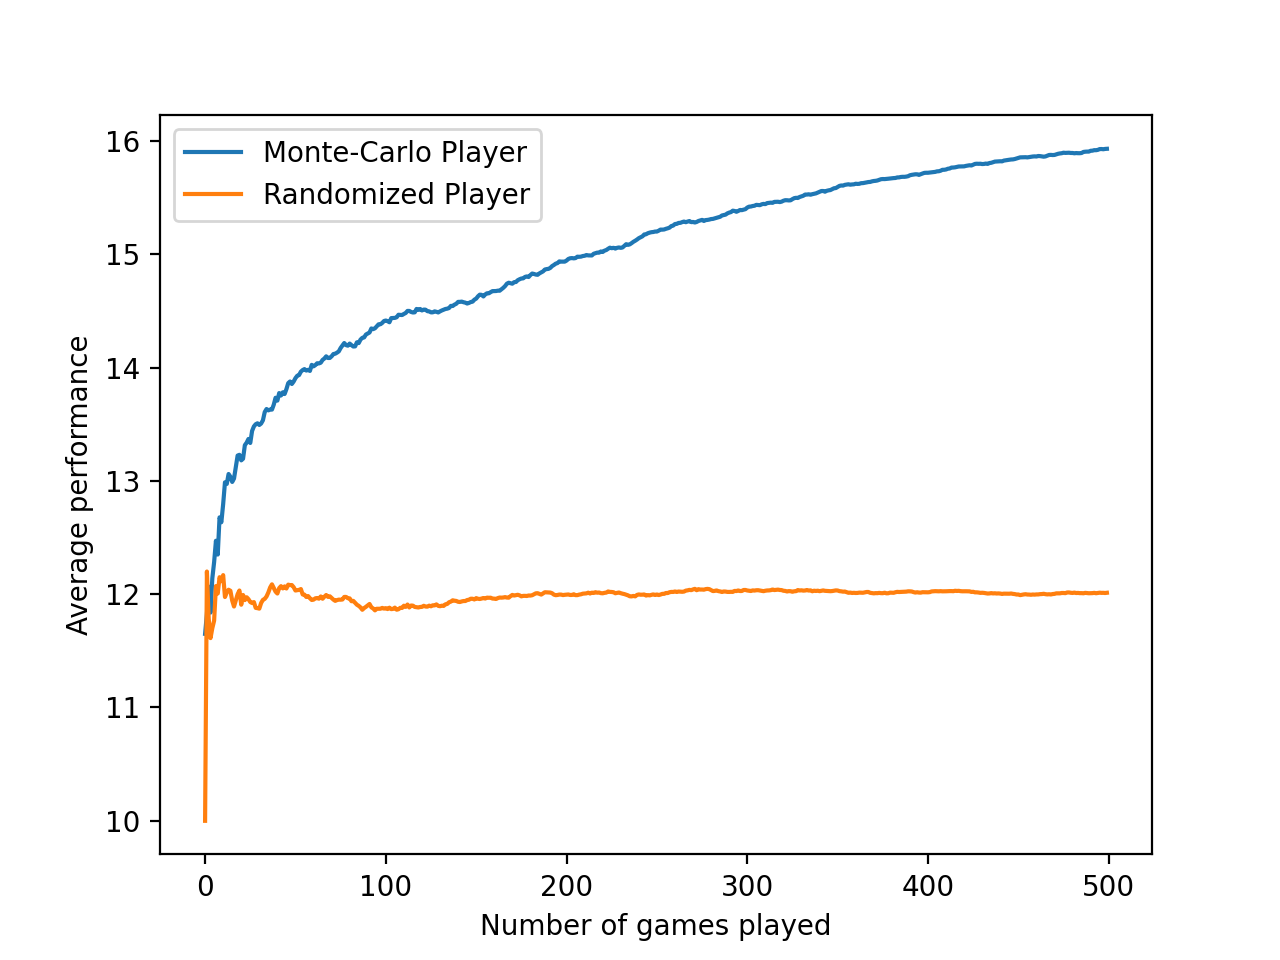
\includegraphics[scale = 0.6]{1.png}
  \caption{results of Monte-Carlo agent (blue line) and randomized agent (red line) play agent the heuristic agent }
\end{figure}

\section{Acknoledgement}
To conduct the experiments I have used the framework for reversi game that Sasha and I developed for our final project. And the experiments and this report are solely my work

\end{document}

